\documentclass[a4paper,12pt]{article}
\usepackage[left=2.50cm,right=2.50cm,top=2cm,bottom=2cm]{geometry}
\usepackage{graphicx,amssymb,amsfonts,amsmath,amsthm,booktabs}

\begin{document}
	\title{2019}
	\author{MCM/ICM}
	\date{summary sheet}
	\maketitle
	\tableofcontents
	\newpage
	\begin{abstract}
T he severe hurricane hit Puerto Rico affected millions of heart. Designing a transportable
disaster response system called “DroneGo.” is an excellent idea to solve such problems. We
used mathematical modeling methods to study the issues involved in packing, site selection,
configuration, and flight planning.

F or the delivery of the system "DroneGo." to Puerto Rico, we simulated the idea that people
always try to ensure a relatively "flat" when packing, and designed a 0 1 programming model
with the goal of maximizing the overall space utilization of the container. Intelligent heuristic

	\textbf{Key words: 3D container load, 0 1 programming, }
	
	\end{abstract}
	\section{Introduction}
	\subsection{Background}
In 2017, the worst hurricane to ever hit the United States territory of Puerto Rico left the
island with severe damage and caused over 2900 fatalities.

At present, drones have been widely used in many fields, including the film and television
industry, traffic supervision, accident relief, etc. As long as the corresponding rules and
	\subsection{Restatement of the problem}
There are some standard dry cargo contain
er and three different medical packages referred
to as MED1,MED2, and MED3.
	\begin{enumerate}
		\item Design each container configuration using a maximum of three containers.
		\item Determining the best location for three cargo containers to enable medical supply delivery
		and video reconnaissance of the road network s.
	\end{enumerate}
	\section{Analysis of Specific Issues}
	\subsection{Question A}
	This
	questions asked us to suggest a Dronego disaster response system for a fleet of drones
	and a medical kit to help the company.
	\subsection{Question B}
	Problem B requires us to determine the optimal location for 1 to 3 cargo container s. In this
	regard, we first perform performance analysis on various types of drones ,
	\section{Assumptions \& Symbols}
	\subsection{Assumptions}
	\begin{enumerate}
		\item In the process of drone transportation, the influence of wind direction and wind direction
		on it is not considered;
		\item Regardless of the impact of altitude;
		\item Ignore the impact of drones slowing down flight speed due to increased loa
	\end{enumerate}
	\subsection{Symbols}
	\begin{table}[!h]
		\centering
		\caption{symbols}
		\label{tab:significance}
		\begin{tabular}{cccc}
			\toprule[0.15em]
			$p$ & Space occupancy ratio &  &  \\
			\midrule[0.3em]
			$\left(l_{i_{1}}, w_{i_{1}}, h_{i_{1}}\right)$ & Medical package size &  & $i_{1}=1,2, \ldots, m$ \\
			$\left(L_{i_{2}}, w_{i_{2}}, H_{i_{2}}\right)$ & Drone Cargo Bay size & in & $\tilde{l}_{2}=1,2, \ldots, n$ \\
			\bottomrule[0.15em]
		\end{tabular}
	\end{table}
	\section{Models}
	\subsection{Analysis and Solving of Question A}
	Question A requires us to design a packaging configuration for up to three standard
	containers and ship them to Puerto Rico for medical supplies.
	\subsubsection{Model Establishment}
	Because the hurricane has caused severe disasters everywhere and the demand for medical
	kits is high, we should try our best to meet the demand for medical kits. Therefore
	
	The specific planning process is as follows:
	\begin{enumerate}
		\item Objective function:
		
		First, we introduce the 0-1 variable to represent the packing selection.
		
		Then, the maximum comprehensive space occupation ratio of medical package to Cargo
		compartment,
	\begin{equation}
	\operatorname{Max} \rho=\alpha \times \sum_{i_{2}=1}^{n} \sum_{i_{1}=1}^{m} \frac{l_{i_{1}} w_{i_{1}} h_{i_{1}} x_{i_{1} i_{2}}}{L_{i_{2}} W_{i_{2}} H_{i_{2}}}+(1-\alpha) \times\left[\sum_{i_{4}=1}^{n} \sum_{i_{2}=1}^{n} \frac{L_{i_{2}} W_{i_{2}} H_{i_{2}} y_{i_{2} i_{4}}}{A_{i_{4}} B_{i_{4}} C_{i_{4}}}+\sum_{i_{4}=1}^{3} \sum_{i_{3}=1}^{q} \frac{a_{i_{3}} b_{i_{3}} c_{i_{3}} z_{i_{3} i_{4}}}{A_{i_{4}} B_{i_{4}} C_{i_{4}}}\right]
	\end{equation}
		\item Constraints
		After getting the objective function, we analyze the constraints of the objective function.
	\begin{enumerate}
		\item Quantity conservation constraints
		Suppose the total number of medical packages placed is m, the total number of Drone
		Cargo Bay used is n and the number of shipping containers is q.
	\begin{equation}
	\sum_{i_{2}=1}^{n} \sum_{i_{1}=1}^{m} x_{i_{1} i_{2}}=\sum_{j=1}^{3} m_{j}=m
	\end{equation}
	In the same way, we will ensure the conservation of the quantity of cargo compartments
	and containers before and after placement:
		\item Basic boxing constraints
		In solving the three-dimensional packing problem, the condition to be satisfied is that after
		the item is placed in the box, t
	\end{enumerate}
	\begin{figure}
		\centering
		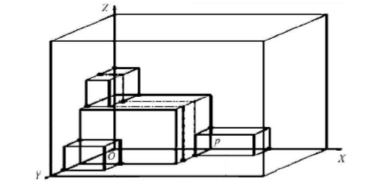
\includegraphics[width=0.5\linewidth]{1}
		\caption{Coordinate system diagram}
		\label{fig:1}
	\end{figure}
	To ensure that it does not exceed the size range of the large box when place, We add 12
	constraints, see the model.
	\end{enumerate}
	According to the above analysis, the 3D packing model is as follows:
	\begin{equation*}
	\operatorname{Max} \rho=\alpha \times \sum_{i_{2}=1}^{n} \sum_{i_{1}=1}^{m} \frac{l_{i} w_{i_{1}} h_{i_{1}} x_{i_{1} i_{2}}}{L_{i_{2}} W_{i_{2}} H_{i_{2}}}+\beta \times\left[\sum_{i_{4}=1}^{3} \sum_{i_{2}=1}^{n} \frac{L_{i_{2}} W_{i_{2}} H_{i_{2}} y_{i_{2} i_{4}}}{A_{i_{4}} B_{i_{4}} C_{i_{4}}}+\sum_{i_{4}=1}^{3} \sum_{i_{3}=1}^{q} \frac{a_{i_{3}} b_{i_{3}} c_{i_{3}} z_{i_{3} i_{4}}}{A_{4} B_{i_{4}} C_{i_{4}}}\right]	
	\end{equation*}
	\begin{figure}
		\centering
		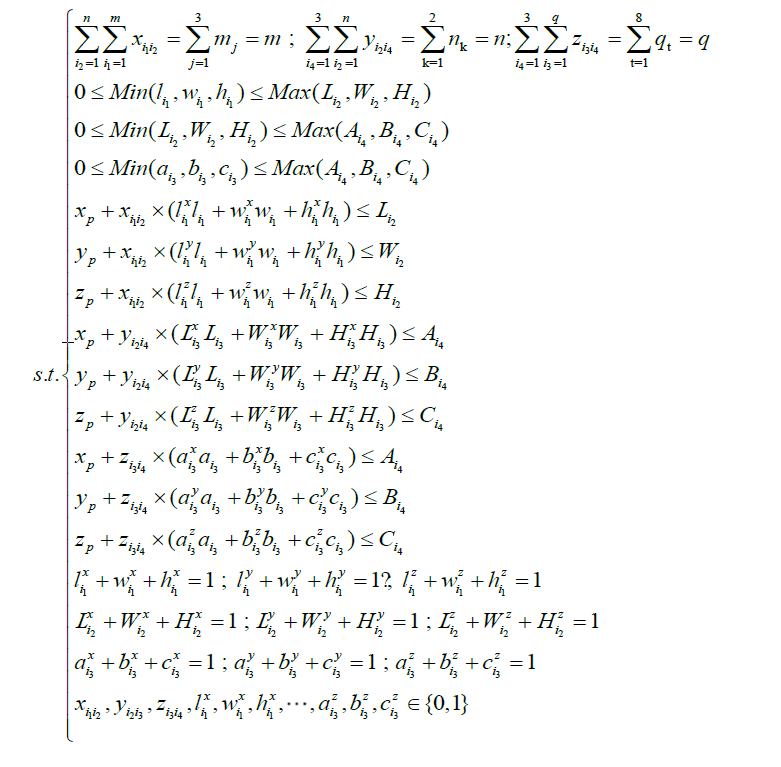
\includegraphics[width=0.7\linewidth]{2}
		\caption{}
	\end{figure}
	\subsubsection{Model Establishment}
	Because the hurricane has caused severe disasters everywhere and the demand for medical
	kits is high,
	\begin{equation}
	\sum_{i_{4}=1}^{3} \sum_{i_{3}=1}^{q} z_{i_{3} i_{4}}=\sum_{i=1}^{8} q_{\mathrm{t}}=q\\
	\end{equation}
	\begin{equation}
	\sum_{i_{4}=1}^{3} \sum_{i_{3}=1}^{q} z_{i_{3} i_{4}}=\sum_{i=1}^{8} q_{\mathrm{t}}=q
	\end{equation}
		\begin{equation}
		0 \leq \operatorname{Min}\left(l_{i_{1}}, w_{i_{1}}, h_{i_{1}}\right) \leq \operatorname{Max}\left(L_{i_{2}}, W_{i_{2}}, H_{i_{2}}\right)\\
	\end{equation}
	\begin{equation}
	0 \leq \operatorname{Min}\left(L_{i_{2}}, W_{i_{2}}, H_{i_{2}}\right) \leq \operatorname{Max}\left(A_{i_{4}}, B_{i_{4}}, C_{i_{4}}\right)
	\end{equation}
	Cargo Bay compartment along the x-axis $l_{i_{1}}^{y}, w_{i_{1}}^{y}, h_{i_{1}}^{y}, l_{i_{1}}^{z}, w_{i_{1}}^{z}, h_{i_{1}}^{z}, L_{i_{3}}^{x}, W_{i_{3}}^{x}, H_{i_{3}}^{x}, L_{i_{3}}^{y}, W_{i_{3}}^{y}$
	\begin{figure}
		\centering
		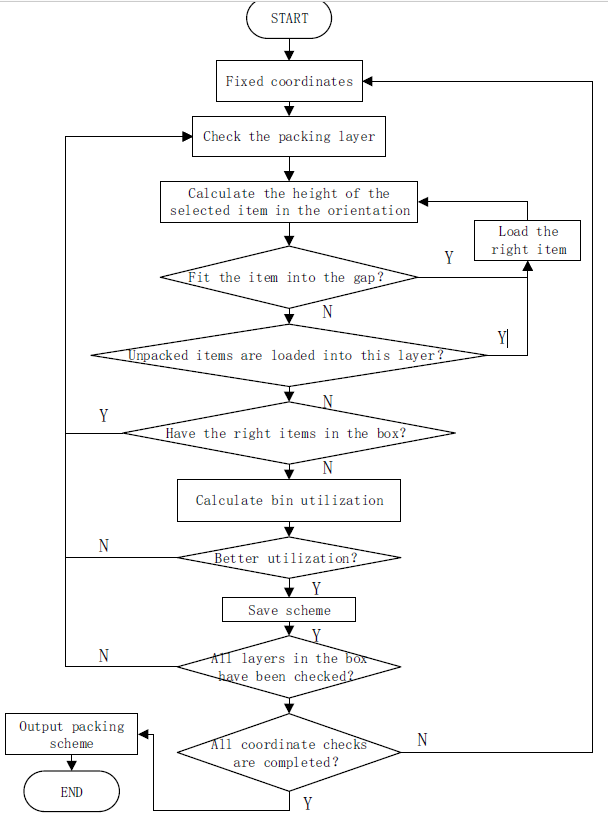
\includegraphics[width=0.7\linewidth]{3}
		\caption{Intelligent Heuristic Approach}
		\label{fig:3}
	\end{figure}
	\begin{enumerate}
		\item First, we use genetic algorithms to write matlab programs(See Appendix 6 for detailed
		procedures.)to find out the combination of goods packing
		
		\textbf{Step l} encodes and initializes the solution space (set the upper and lower bounds of the
		total number of Drone Cargo Bay);
		
		\textbf{Step 2} initialize population
	\end{enumerate}
	\begin{equation}
	D=\left[\begin{array}{cccccc}
	{}  & {A} & {B} & {C} & {D} & {E} \\
	{Caribbean  \text {Medical Center A}}  & {0} & {} & {} & {} & {} \\
	{\text {Hospital HIMB A}}  & {41.99} & {0} & {} & {} & {}  \\
	{\text {Hospital Pavia Santurce C}} & {46.03} & {24.85} & {0} & {}  & {} \\
	{\text {Puerto Rico Children's Hospital D}}  & {54.44} & {24.30} & {10.50} & {0} & {} \\
	 {\text {Hospital Pavia Arecibo E} } & {115.14} & {79.03} & {69.77} & {60.70} & {0}
	\end{array}\right]
	\end{equation}
	
	\begin{align}
		x^4 & = y \notag \\
		x^6 & = y
	\end{align}
	\begin{equation}
	\min \quad \operatorname{mum}=\sum_{k=1}^{3} \sum_{i=1}^{7} x_{k i}
	\end{equation}
	
	\begin{equation}
	T_{1} \leq \frac{f_{B}}{2}, T_{2} \leq \frac{f_{B}}{2}, T_{3} \leq \frac{f_{F}}{2}, T_{4} \leq \frac{f_{B}}{2}, T_{5} \leq \frac{f_{B}}{2}
	\end{equation}
\end{document}